\section{Deep Information Propagation in DGN}\label{sec:optimisation}

\begin{assumption}\label{assmp:main}
i) $\Tv_0\stackrel{iid}\sim Ber\left(\frac{1}{2}\right)$ over the set $\{-\sigma,+\sigma\}$. ii) $\G_0$ is statistically independent of $\Theta_0$.
\end{assumption}
 \Cref{assmp:main} can be satisfied by two interesting gating schemes namely \emph{fixed-random-gating} (FRG), and \emph{decoupled gating}. In FRG we are looking at the DGN $\N(\G_{\dagger};\Tv_t)$, i.e., corresponding to each of the $n$ input examples, random gating patterns are generated by sampling the gating values from $Ber(\mu)$ and collected in $\G_0$ which is kept constant through training. In \emph{decouple gating} we are looking at the DGN denoted by $\N(\Tg_\dagger, \infty;\Tv_t)$ (these are also known as gated linear unit or GaLU networks), where $\Tg_0\in \R^{d_{net}}$ is initialised at random and statistically independent of $\Tv_0\in \R^{d_{net}}$ which is initialised according to \Cref{assmp:main}. It follows that DGN with FRG cannot generalise, while the GaLU networks can generalise. 
 
\begin{theorem}[DIP]\label{th:opti} Let $\kappa_t(s,s',i)\stackrel{def}=\underset{p_1,p_2\rsa i}{\sum_{p_1,p_2\in P:}} A_{\G_t}(x_s,p_1) A_{\G_t}(x_{s'},p_2) \ip{\varphi_{t,p_1}, \varphi_{t,p_2}}$. 
$(A)$ The Gram matrix $K_t$ is then given by ${K_t(s,s')}=\sum_{i=1}^{d_{in}} x(i,s)x(i,s') \kappa_t(s,s',i)$. 

Further, under Assumption~\ref{assmp:main} it follows that:

$(B)$ For paths $p,p_1,p_2\in \P, p_1\neq p_2$, at initialisation we have  i) $\E{\ip{\varphi_{0,p_1}, \varphi_{0,p_2}}}= 0$ and ii)${\ip{\varphi_{0,p}, \varphi_{0,p}}}= d\sigma^{2(d-1)}$.

Under further condition that $\frac{4d}{w^2}<1$, it follows that:

$(C)$ $\E{K_0}=d\sigma^{2(d-1)}(x^\top x \odot \lambda_0)$.

$(D)$ $Var\left[K_0\right]\leq O\left(d^2_{in}\sigma^{4(d-1)}\max\{d^2w^{2(d-2)+1}, d^3w^{2(d-2)}\}\right)$.
\end{theorem}
\textbf{Discussion:}

$\bullet$  \textbf{Signal-Wire Separation:} Note that $\kappa_t$ in \Cref{th:opti}-$(A)$ term encodes the \emph{wire}, i.e., the effect of gradient flow within the network in terms of path sensitivities (see discussion on first order path term in \Cref{sec:notation}). Further, note that in the expression for $K_t$, the signal term, i.e., $x_s(i)x_{s'}(i)$, which is the interaction of the $i^{th}$ dimension of the input gets separated from the $\kappa_t$ term.

$\bullet$ \textbf{Disentangling the paths:} Thanks to \Cref{assmp:main}, inter-path sensitivities in $\kappa_0$ cancel out each other in \Cref{th:opti}-$(B)$, and only the self-terms remain which shows up as the $\lambda_0$ in the right-hand side of the expression for $\E{K_0}$ in \Cref{th:opti}-$(C)$.
 
$\bullet$ \textbf{Increasing depth whitens $K_0$:} In the case of FRG, $\bar{\lambda}_{self}=\mathbb{E}_{\mu}\left[\lambda_0(s,s)\right]=(\mu w)^{d-1}$, $\bar{\lambda}_{cross}=\mathbb{E}_{\mu}\left[\lambda_0(s,s')\right]= (\mu^2w)^{d-1}$, and hence for $\sigma=\sqrt{\frac{1}{\mu w}}$, the decay of the non-diagonal terms is at an uniform rate given by $\mu^{d-1}$. Thus increasing depth leads to whitening of the Gram matrix $K_0$. A similar argument can be made for the case of GaLU networks, except that the each non-diagonal element of $\E{K_0}/d$ decays at a different exponential rate, however, since $n$ is finite one can always obtain an uniform exponential decay rate as an upper bound. Thus for a large enough width, as depth increases, the $K_0/d$ approaches an identity matrix.

$\bullet$ \textbf{Too much depth hurts:} Note that for $\sigma=O\left(\sqrt{\frac{1}{w}}\right)$, for a fixed depth $d$, as width $w$ increases, $K_0\ra\E{K_0}$. However, the variance expression in \Cref{th:opti}-$(D)$ involves $d^2$ and $d^3$ terms, and hence for a fixed width as depth increases, the entries of $K_0$ deviates from $\E{K_0}$, and as a result the spectrum of $K_0$ degrades, thereby hurting training performance.

\textbf{Experiment 1(Dataset):} Consider the dataset $(x_s,y_s)_{s=1}^n\in \R\times \R$, where $x_s=1,\forall s\in [n]$, and $y_s\sim unif([-1,1])$, $n=200$. The input Gram matrix $x^\top x$ is a $n\times n$ matrix with all entries equal to $1$ and its rank is equal to 1. Since all the inputs are identical, this is the worst possible case for optimisation.

\textbf{Theoretical Prediction:} From \Cref{th:opti}, and the subsequent discussions, it follows that, all the diagonal entries of $\E{K_0}/d$ are $1$ and non-diagonal entries are $\mu^{d-1}$. Now, let $\rho_i\geq 0,i \in [n]$ be the eigenvalues of $\frac{\E{K_0}}{d}$, and let $\rho_{\max}$ and $\rho_{\min}$ be the largest and smallest eigenvalues. From the structure of \eqref{eq:mat}, one can easily show that $\rho_{\max}=1+(n-1)\mu^{d-1}$ and corresponds to the eigenvector with all entries as $1$, and $\rho_{\min}=(1-\mu^{d-1})$ repeats $(n-1)$ times, which corresponds to eigenvectors given by $[0, 0, \ldots, \underbrace{1, -1}_{\text{$i$ and $i+1$}}, 0,0,\ldots, 0]^\top \in \R^n$ for $i=1,\ldots,n-1$.

\begin{comment}
\begin{figure}[h]
\resizebox{\columnwidth}{!}{
\begin{tabular}{cc}
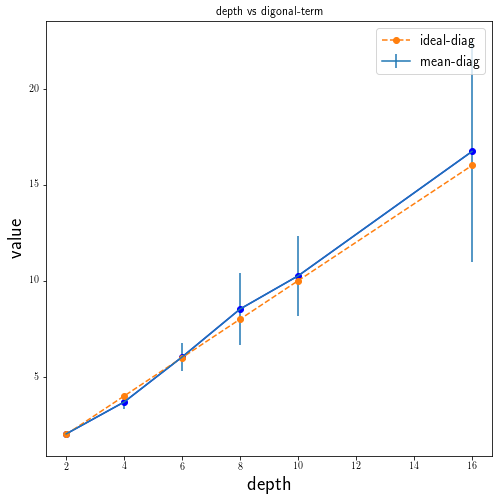
\includegraphics[scale=0.4]{figs/dgn-frg-diag.png}
&
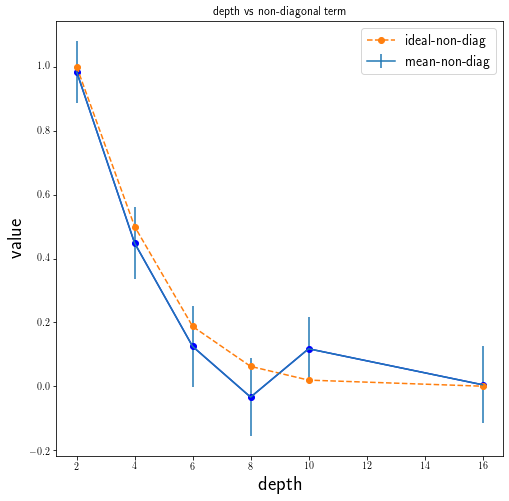
\includegraphics[scale=0.4]{figs/dgn-frg-non-diag.png}
\end{tabular}
}
\caption{For $w=500$, and $\mu=0.5$, (an arbitrary) diagonal (left plot) and non-diagonal (right plot) of the Gram matrix $K_0$ for dataset in Experiment~$1$ is shown. The plots are averaged over $20$ runs.}
\label{fig:dgn-frg-gram-diag}
\end{figure}
\end{comment}
\begin{figure*}
\resizebox{\textwidth}{!}{
\begin{tabular}{ccccc}
%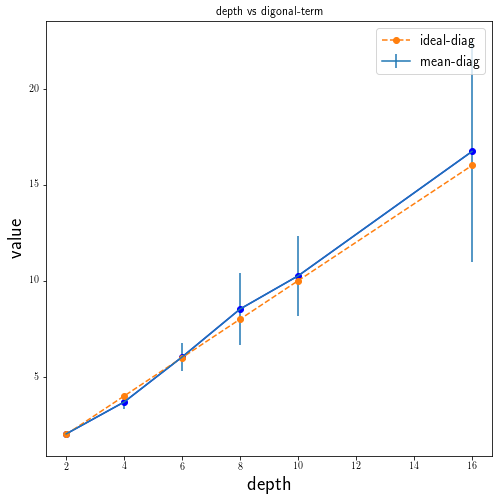
\includegraphics[scale=0.4]{figs/dgn-frg-diag.png}
%&
%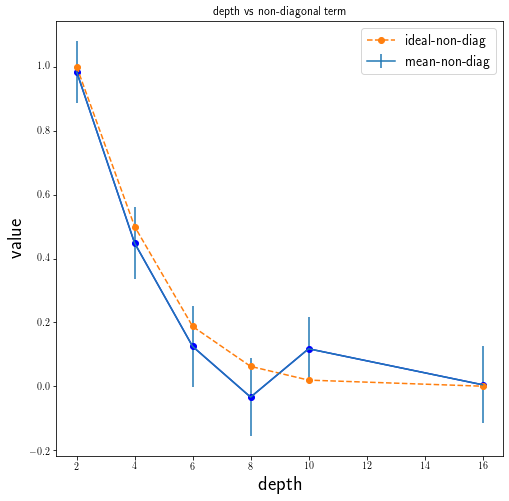
\includegraphics[scale=0.4]{figs/dgn-frg-non-diag.png}

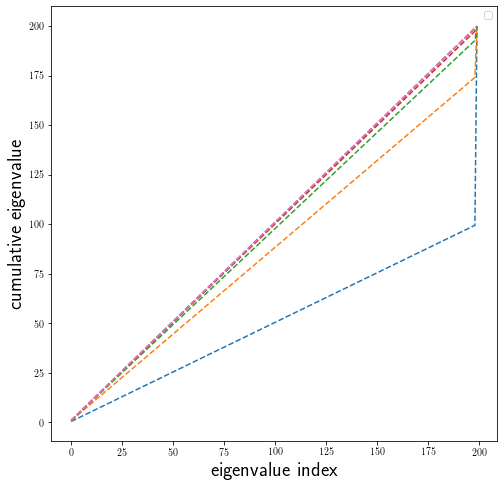
\includegraphics[scale=0.4]{figs/dgn-fra-ecdf-ideal.png}
&
%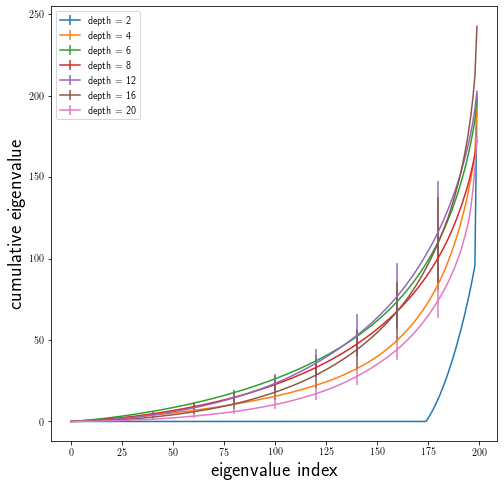
\includegraphics[scale=0.4]{figs/dgn-fra-ecdfbyd-w25.png}
&
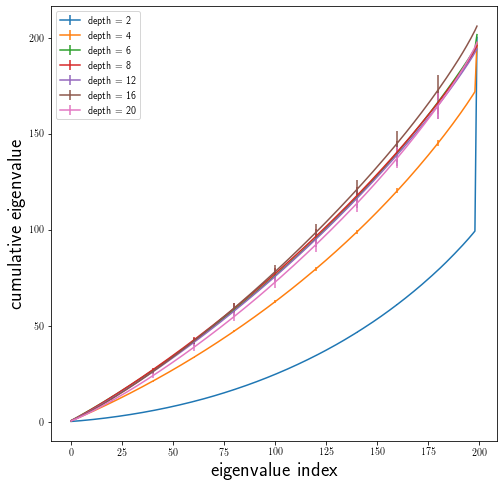
\includegraphics[scale=0.4]{figs/dgn-fra-ecdfbyd-w500.png}
&
%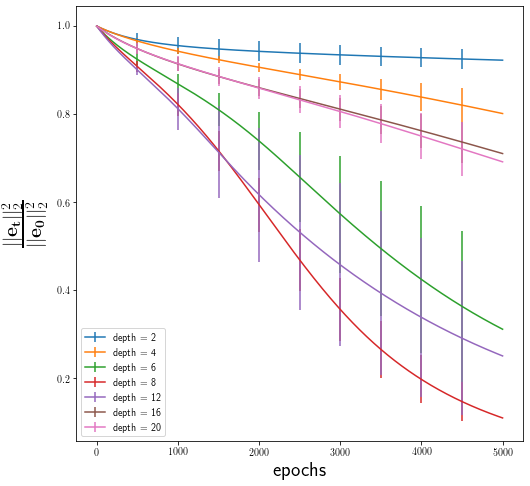
\includegraphics[scale=0.4]{figs/dgn-fra-conv-w25.png}
&
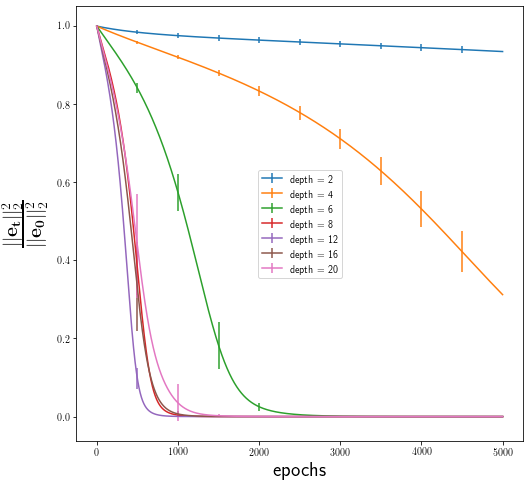
\includegraphics[scale=0.4]{figs/dgn-fra-conv-w500.png}
%&
%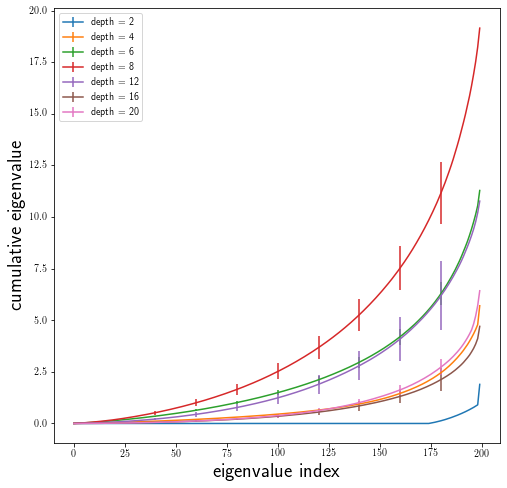
\includegraphics[scale=0.4]{figs/dgn-fra-ecdfbymax-w25.png}
%&
%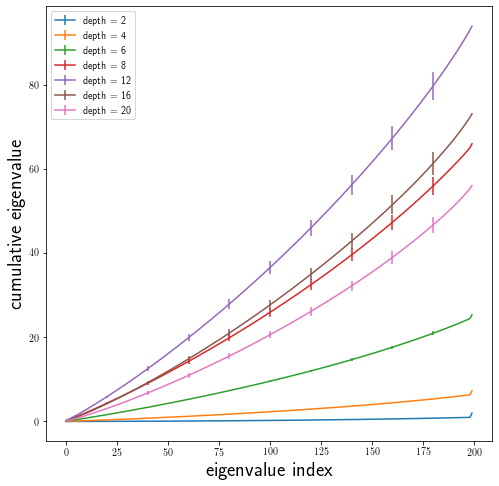
\includegraphics[scale=0.4]{figs/dgn-fra-ecdfbymax-w500.png}
\end{tabular}
}
\caption{Shows the plots for DGN-FRG with $\mu=\frac{1}{2}$ and $\sigma=\sqrt{\frac{2}{w}}$. The first plot in the left shows the ideal cumulative eigenvalue (e.c.d.f) for various depths $d=2,4,6,8,12,16,20$. Note that the ideal plot converges to identity matrix as $d$ increases. The second plot from the left shows the cumulative eigenvalues (e.c.d.f) for $w=500$. }
\label{fig:dgn-frg-gram-ecdf}
\end{figure*}
\textbf{Numerical Evidence:} We look at the cumulative eigenvalue (e.c.d.f) obtained by first sorting the eigenvalues in ascending order then looking at their cumulative sum. The ideal behaviour (middle plot of \Cref{fig:dgn-frg-gram-ecdf}) as predicted from theory is that for indices $k\in[n-1]$, the e.c.d.f should increase at a linear rate, i.e., the cumulative sum of the first $k$ indices is equal to $k(1-\mu^{d-1})$, and the difference between the last two indices is $1+(n-1)\mu^{d-1}$. In \Cref{fig:dgn-frg-gram-ecdf}, we plot the e.c.d.f for various depths $d=2,4,6,8,12,16,20$ and $500$. 

In order to compare how the rate of convergence varies with the depth in DGN-FRG network, we set the step-size $\alpha=\frac{0.1}{\rho_{\max}}$, $w=100$. We use the vanilla SGD-optimiser. Note that if follows from \eqref{eq:basictraj} that the convergence rate is determined by a linear recursion, and choosing $\alpha=\frac{0.1}{\rho_{\max}}$ can be seen to be equivalent to having a constant step-size of $\alpha=0.1$ but dividing the Gram matrix by its maximum eigenvalue instead. Thus, after this rescaling, the maximum eigenvalue is $1$ uniformly across all the instances, and the convergence should be limited by the smaller eigenvalues. We also look at the convergence rate of the ratio $\frac{\norm{e_t}^2_2}{\norm{e_0}^2_2}$, and we observe that the convergence rate gets better with depth as predicted by theory (\Cref{fig:dgn-frg}).


\begin{comment}
In the case of GaLU networks, we can define $\bar{\lambda}_{self}(s)\stackrel{def}=\mathbb{E}_{\Tg_0}\left[\lambda_0(s,s)\right]$, and $\bar{\lambda}_{cross}(s,s')\stackrel{def}= \mathbb{E}_{\Tg_0}\left[\lambda_0(s,s')\right]$. Note that, due to the inherent symmetry in weights (Assumption~\ref{assmp:mainone}) , we can expect roughly half the number of activations to be \emph{on}, and it follows that $\bar{\lambda}_{self}(s)\approx (\mu w)^{d-1}$ with $\mu\approx\frac12$. Also, let $\tau(s,s',l)\stackrel{def}=\sum_{i=1}^w G_{x_s,t}(l,i)G_{x_{s'},t}(l,i)$,  let $\eta\stackrel{def}=\max_s\left(\max_{s',l} \frac{\tau(s,s',l)}{\tau(s,s,l)}\right)$ be the maximum overlap between gates of a layer (maximum taken over over input pairs $s,s'\in[n]$ and layers $l\in [d]$), then it follows that $\max_{s,s'\in [n]} \frac{\bar{\lambda}_{cross}(s,s')}{\bar{\lambda}_{self}(s)}\leq \eta^{d-1}$. Thus, by setting $\sigma=\sqrt{\frac{1}{\mu w}}$  we can see that the non-diagonal entries of the $\E{K_0}/d$ decay at a rate upper bounded by $\eta^{d-1}$. 
\end{comment}
\begin{comment}
\textbf{Choice of $\sigma$:} Note that, in the case of gates taking values in $\{0,1\}$, $\lambda_0(s,s'), s,s'\in [n]$ is a measure of overlap of sub-networks that start at any given input node, end at the output node, and are active for both input examples $s,s'$.
Loosely speaking, say, in each layer $\mu\in(0,1)$ fraction of the gates are \emph{on}, then $\lambda_0(s,s)$ is about $(\mu w)^{d-1}$. Thus, to ensure that the signal does not blow up in a DGN, we need to ensure $(\sigma^2 \mu w)^{d-1}=1$, which means $\sigma=O\left(\sqrt{\frac1{\mu w}}\right)$. %In our experiments, we set $\sigma=\sqrt{\frac{2}{w}}$.

In the expression for $\E{K_0}$, note that the input Gram matrix $x^\top x \in \R^{n\times n}$ is separate from $\lambda_0\in \R^{n\times n}$,	 which is a Gram matrix of the active sub-networks. Thanks to the path-view, we do not lose track of the input information, which, is otherwise bound to happen if we were to choose a layer by layer view of DIP in DGNs.




\textbf{Fixed Random Gating (DGN-FRG)} involves sampling the gates $\G_0$ from $Ber\left(\mu\right)$, and hence there is a random sub-network which is active for each input. Under FRG, we can obtain closed form expression for the `$\lambda(\cdot,\cdot,\cdot)$' term as below:

\begin{lemma}\label{lm:dgn-fra}  
 Under Assumption~\ref{assmp:mainone},~\ref{assmp:maintwo} and gates sampled iid $Ber(\mu)$, we have, $\forall s,s'\in[n]$

(i) $\mathbb{E}_p\left[\lambda_0(s,s)\right]=\bar{\lambda}_{self}=(\mu w)^{d-1}$

ii) $\mathbb{E}_p\left[\lambda_0(s,s')\right]=\bar{\lambda}_{cross}= (\mu^2w)^{d-1}$
\end{lemma}

\textbf{DIP in DGN-FRG:} For $\sigma=\sqrt{\frac{1}{\mu w}}$, we have:

\begin{align*}
\frac{\E{K_0}}{d}=\left[\begin{matrix}
\cdot&\cdot &\cdot &\cdot &\cdot \\ 
\cdot&\ip{x_s,x_s}\quad\quad &\cdot &\quad\quad\ip{x_s,x_{s'}}\mu^{d-1} &\cdot\\ 
\cdot&\ip{x_{s'},x_s}\mu^{d-1} &\cdot &\ip{x_{s'},x_{s'}} &\cdot \\
\cdot&\cdot &\cdot &\cdot &\cdot  
\end{matrix}\right]
\end{align*}


\textbf{Experiment $1$:} Consider the dataset $(x_s,y_s)_{s=1}^n\in \R\times \R$, where $x_s=1,\forall s\in [n]$, and $y_s\sim unif([-1,1])$, $n=200$. The input Gram matrix $x^\top x$ is a $n\times n$ matrix with all entries equal to $1$ and its rank is equal to 1. Since all the inputs are identical, this is the worst possible case for optimisation.


\textbf{Why increasing depth till a point helps ?} 
In the case of \textbf{Experiment $1$}, we have:

\begin{align}\label{eq:mat}
\frac{\E{K_0}}{d}=\left[\begin{matrix}
1 &\mu^{d-1} &\ldots &\mu^{d-1} &\ldots\\ 
\ldots &1 &\ldots &\mu^{d-1} &\ldots\\ 
\ldots &\mu^{d-1} &\ldots &1 &\ldots \\
\ldots &\mu^{d-1} &\ldots &\mu^{d-1} &1\\ 
\end{matrix}\right]
\end{align}

i.e., all the diagonal entries are $1$ and non-diagonal entries are $\mu^{d-1}$. Now, let $\rho_i\geq 0,i \in [n]$ be the eigenvalues of $\frac{\E{K_0}}{d}$, and let $\rho_{\max}$ and $\rho_{\min}$ be the largest and smallest eigenvalues. From the structure of \eqref{eq:mat}, one can easily show that $\rho_{\max}=1+(n-1)\mu^{d-1}$ and corresponds to the eigenvector with all entries as $1$, and $\rho_{\min}=(1-\mu^{d-1})$ repeats $(n-1)$ times, which corresponds to eigenvectors given by $[0, 0, \ldots, \underbrace{1, -1}_{\text{$i$ and $i+1$}}, 0,0,\ldots, 0]^\top \in \R^n$ for $i=1,\ldots,n-1$.



\textbf{Why increasing depth beyond a point hurts?} 
In \Cref{th:dgnexp}, note that for a fixed width $w$, as the depth increases, the variance of $K_0(s,s')$ increases, and hence the entries of $K_0$ deviates from its expected value $\E{K_0}$. Thus the structure of the Gram matrix degrades from \eqref{eq:mat}, leading to smaller eigenvalues.

\textbf{Numerical Evidence (Gram Matrix):} We fix arbitrary diagonal and non-diagonal entries, and look at their value averaged over $20$ run (see \Cref{fig:dgn-frg-gram-diag}). The actual values shown in bold indeed follow the ideal values shown in the dotted lines and the values are as per \eqref{eq:mat}). 


\begin{figure}[h]
\resizebox{\columnwidth}{!}{
\begin{tabular}{cc}
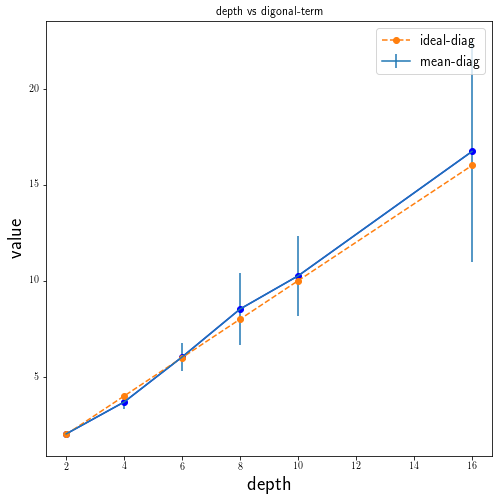
\includegraphics[scale=0.4]{figs/dgn-frg-diag.png}
&
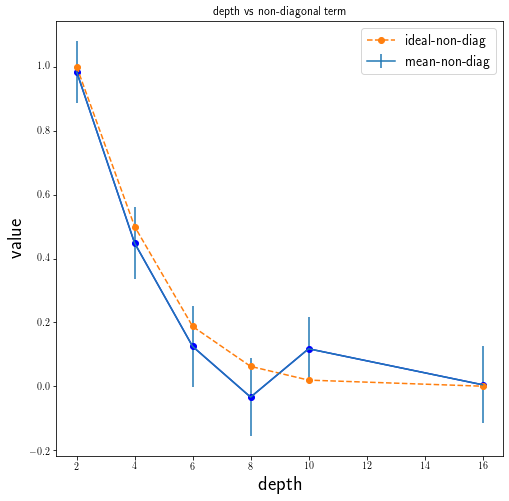
\includegraphics[scale=0.4]{figs/dgn-frg-non-diag.png}
\end{tabular}
}
\caption{For $w=500$, and $\mu=0.5$, (an arbitrary) diagonal (left plot) and non-diagonal (right plot) of the Gram matrix $K_0$ for dataset in Experiment~$1$ is shown. The plots are averaged over $20$ runs.}
\label{fig:dgn-frg-gram-diag}
\end{figure}


\textbf{Numerical Evidence (Spectrum):} 
Next, we look at the cumulative eigenvalue (e.c.d.f) obtained by first sorting the eigenvalues in ascending order then looking at their cumulative sum. The ideal behaviour (middle plot of \Cref{fig:dgn-frg-gram-ecdf}) as predicted from theory is that for indices $k\in[n-1]$, the e.c.d.f should increase at a linear rate, i.e., the cumulative sum of the first $k$ indices is equal to $k(1-\mu^{d-1})$, and the difference between the last two indices is $1+(n-1)\mu^{d-1}$. In \Cref{fig:dgn-frg-gram-ecdf}, we plot the e.c.d.f for various depths $d=2,4,6,8,12,16,20$ and two different width namely $w=25,500$. It can be seen that as $w$ increases, the difference between the ideal and actual e.c.d.f curves is less ($w=500$ when compared to $w=25$).

\textbf{Numerical Evidence (Role of Depth):} 
In order to compare how the rate of convergence varies with the depth in DGN-FRG network, we set the step-size $\alpha=\frac{0.1}{\rho_{\max}}$, $w=100$, and fit the data described in \textbf{Experiment $1$}. We use the vanilla SGD-optimiser. Note that if follows from \eqref{eq:basictraj} that the convergence rate is determined by a linear recursion, and choosing $\alpha=\frac{0.1}{\rho_{\max}}$ can be seen to be equivalent to having a constant step-size of $\alpha=0.1$ but dividing the Gram matrix by its maximum eigenvalue instead. Thus, after this rescaling, the maximum eigenvalue is $1$ uniformly across all the instances, and the convergence should be limited by the smaller eigenvalues. We also look at the convergence rate of the ratio $\frac{\norm{e_t}^2_2}{\norm{e_0}^2_2}$, and we observe that the convergence rate gets better with depth as predicted by theory (\Cref{fig:dgn-frg}).

\begin{figure*}
\resizebox{\textwidth}{!}{
\begin{tabular}{cccc}

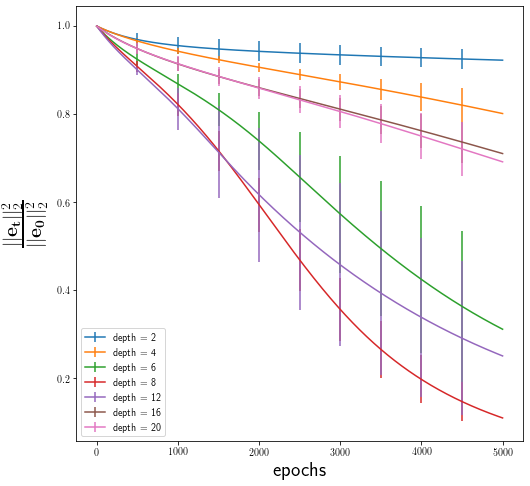
\includegraphics[scale=0.4]{figs/dgn-fra-conv-w25.png}
&
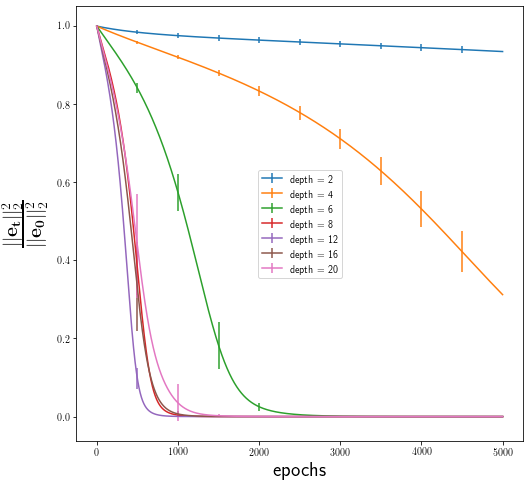
\includegraphics[scale=0.4]{figs/dgn-fra-conv-w500.png}
&
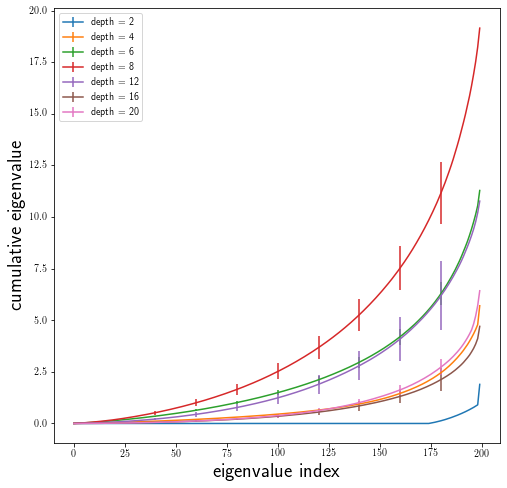
\includegraphics[scale=0.4]{figs/dgn-fra-ecdfbymax-w25.png}
&
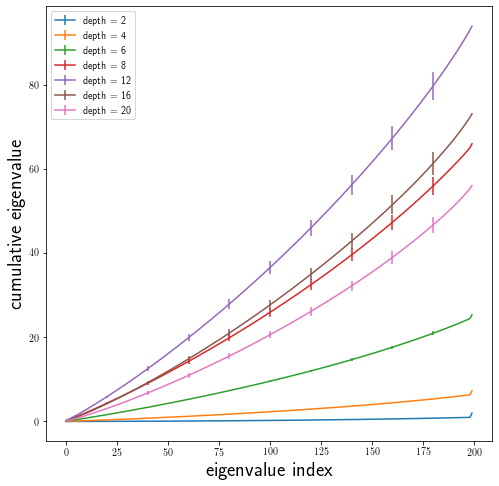
\includegraphics[scale=0.4]{figs/dgn-fra-ecdfbymax-w500.png}
\end{tabular}
}
\caption{Shows the plots for DGN-FRG. The left two plots show the convergence rates for $w=25$ and $w=500$. The right two values are showing the e.c.d.f obtained by first dividing the Gram matrix by their maximum eigenvalue. The plots are averaged over $5$ runs.}
\label{fig:dgn-frg}
\end{figure*}
\begin{figure*}
\resizebox{\textwidth}{!}{
\begin{tabular}{cccc}
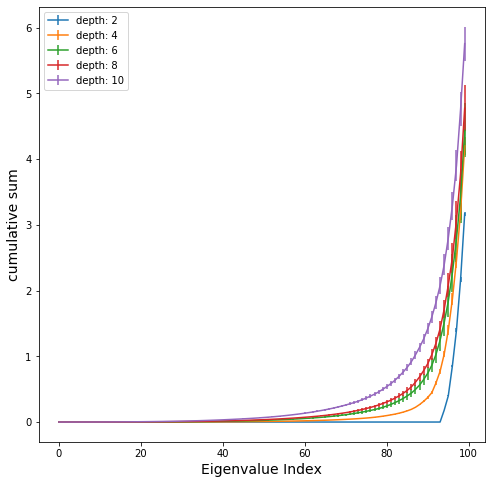
\includegraphics[scale=0.4]{figs/galu-ecdf-d.png}
&
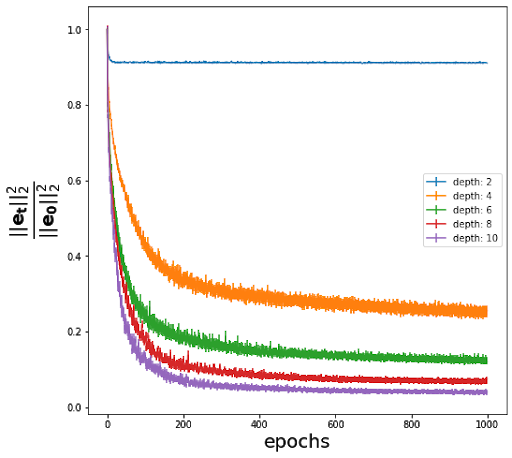
\includegraphics[scale=0.4]{figs/galu-conv-d.png}
&
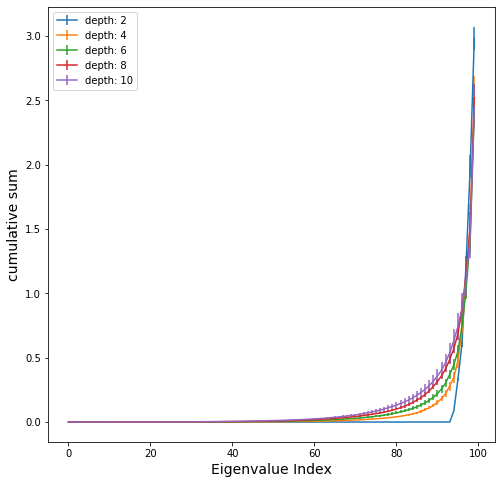
\includegraphics[scale=0.4]{figs/relu-ecdf.png}
&
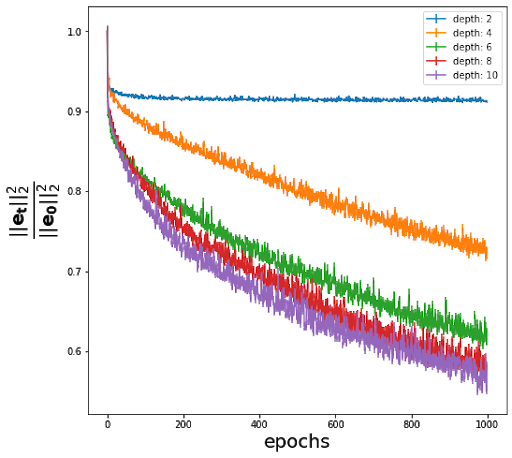
\includegraphics[scale=0.4]{figs/relu-conv.png}
\end{tabular}
}
\caption{The left two plots shows the e.c.d.f and convergence rates for various depth in GaLU networks $w=100$. The third and fourth plot from the left show the e.c.d.f and convergence rates for various depth in ReLU networks $w=100$. The plots are averaged over $5$ runs. }
\label{fig:galu-d}
\end{figure*}

\textbf{GaLU Networks:} Here, the gating values are obtained from a DNN with ReLU activation, parameterised by $\Tg\in \R^{d_{net}}$ (these weights are frozen). Now, let us define $\bar{\lambda}_{self}(s)\stackrel{def}=\mathbb{E}_{\Tg_0}\left[\lambda_0(s,s)\right]$, and $\bar{\lambda}_{cross}(s,s')\stackrel{def}= \mathbb{E}_{\Tg_0}\left[\lambda_0(s,s')\right]$. Note that, due to the inherent symmetry in weights (Assumption~\ref{assmp:mainone}) , we can expect roughly half the number of activations to be \emph{on}, and it follows that $\bar{\lambda}_{self}(s)\approx (\mu w)^{d-1}$ with $\mu\approx\frac12$. Also, let $\tau(s,s',l)\stackrel{def}=\sum_{i=1}^w G_{x_s,t}(l,i)G_{x_s',t}(l,i)$,  let $\eta\stackrel{def}=\max_s\left(\max_{s',l} \frac{\tau(s,s',l)}{\tau(s,s,l)}\right)$ be the maximum overlap between gates of a layer (maximum taken over over input pairs $s,s'\in[n]$ and layers $l\in [d]$), then it follows that $\max_{s,s'\in [n]} \frac{\bar{\lambda}_{cross}(s,s')}{\bar{\lambda}_{self}(s)}\leq \eta^{d-1}$. Thus,  we can see that while the non-diagonal entries of the $\E{K_0}$ decay at a different rates, the rate of decay is nonetheless upper bounded by $\eta^{d-1}$. Note that in DGN-FRG decay of non-diagonal terms is at a uniform rate given by $\mu^{d-1}$.



\textbf{Experiment $2$:} To characterise the optimisation performance of GaLU and ReLU networks, we consider the dataset $(x_s,y_s)_{s=1}^{n}\in \R^2\times \R$, where, $x_s\stackrel{iid}\sim unif(\left[-1,1\right]^2)$ and $y_s\stackrel{iid}\sim unif([-1,1])$, $n=100$. The results are shown in \Cref{fig:galu-d}. The rationale behind choosing this data set is that, we want the inputs to be highly correlated by choice.
 
 \textbf{GaLU Networks (Depth helps in training): }The trend is similar to DGN-FRG case, in that, both e.c.d.f as well as convergence get better with increasing depth. Here too we set the step-size $\alpha=\frac{0.1}{\rho_{\max}}$ (and use vanilla SGD). We also observe that in \textbf{Experiment $2$} \emph{GaLU networks optimise better than standard ReLU networks}, and it is also true that the e.c.d.f for the case of GaLU is better than that of ReLU. This can be attributed to the fact that, in ReLU network the dot product of two different active paths is not zero and hence the Gram matrix entries fall back to the algebraic expression for $K_t$ in \eqref{eq:ktalg}.


\end{comment}